\documentclass[12pt]{article}
\usepackage[utf8]{inputenc}
\usepackage{url}
\usepackage{latexsym,amsfonts,amssymb,amsthm,amsmath}
\usepackage{mathtools}
\usepackage{enumerate}
\usepackage{hyperref} 
\usepackage{graphicx}
\usepackage{subcaption}
\usepackage{float}

% Ajustements des marges
\setlength{\parindent}{0in}       % Pas de retrait au début des paragraphes
\setlength{\oddsidemargin}{-0.3in} % Marges plus étroites
\setlength{\evensidemargin}{-0.3in}
\setlength{\textwidth}{7.2in}     % Largeur de texte augmentée
\setlength{\textheight}{9.7in}    % Hauteur de texte augmentée
\setlength{\topmargin}{-0.7in}    % Réduction de la marge supérieure
\setlength{\headheight}{14pt}     % Hauteur de l'en-tête
\setlength{\headsep}{10pt}        % Espacement entre l'en-tête et le texte
\setlength{\parskip}{2pt}         % Réduction de l'espacement entre paragraphes

% Réduction de l'espacement autour des titres
\usepackage[compact]{titlesec}
\titlespacing*{\section}{0pt}{*1.5}{*1.2} % Espacement avant/après une section
\titlespacing*{\subsection}{0pt}{*1.2}{*1.0}
\titlespacing*{\subsubsection}{0pt}{*1.0}{*0.8}

% Réduction des espaces avant/après les figures
\setlength{\intextsep}{8pt}  % Espace autour des figures flottantes
\setlength{\textfloatsep}{10pt} % Espacement entre texte et figures

% Compactage de la table des matières
\usepackage{tocloft}
\setlength{\cftbeforesecskip}{5pt} % Réduction de l'espacement vertical

% Réduction de l'espacement des items dans les listes
\usepackage{enumitem}
\setlist{nosep, left=0pt}  % Réduction de l'espacement dans les listes

\title{Prédiction structurée pour le traitement automatique de la langue}
\author{Baptiste Chachura (Leader), Bouger Lisa (Follower)}

\begin{document}

\maketitle
\vspace{-0.2in} % Réduction de l'espace après le titre

\tableofcontents
\newpage

% Corps du document
\section{Etiqueteur de super-senses avec transformers pré-entraînés}
L’objectif de ce projet est de développer et d’évaluer un système capable de prédire des super-senses, des étiquettes sémantiques 
de haut niveau, pour des mots dans un corpus annoté (sequoia). Ces étiquettes indiquent la catégorie sémantique gros-grain d’un mot,
comme Feeling pour "surprise" ou Body pour "jambe".

Pour cela nous allons utiliser un modèle pré-entraîné pour la prédiction des embeddings des mots des phrases( ici dans notre cas 
nous utiliserons une architecture BERT et plus précisément les modèles camembert et google-bert), suivis d'un classifieur.

\section{Perceptron Multi Couches}
Dans un premier temps nous allons utiliser un perceptron multi-couches afin de classifier nos embeddings. L'architecture du modèle est choisie
de manière arbitraire et se compose d'une couche d'entrée de la dimension des embeddinds du transformers (ici 768), suivie de deux couches 
de dimension 200 puis une sortie vers une couche de dimension 25 ce qui correspond à notre nombre de super sense + 1 pour les mots sans classe ( annotés par "*"). 
Les différentes couches sont séparées par des Relu.

Nous observons que le tokenizer associé au modèle Bert nous donne parfois plusieurs tokens pour un mot ce qui est problématique car 
dans notre cas nous souhaitons avoir un seul et unique embedding par mot afin de pouvoir prédire son étiquette. Pour palier à cela nous
définissons un dataloader qui à partir des phrases du jeu de données, calcule les embeddings pour chaque token et retourne des embeddings sur les mots en effectuant la 
moyenne des embeddings des token qui constituent le mot.
\subsection{Camembert VS Google-bert}

Les déclinaisons de l'architecture BERT sont nombreuses et leurs performances pas toujours égales ce qui peut avoir une influence non négligeable sur 
les performances de notre classifieur. Pour étudier cela nous allons comparer deux modèles pour la génération de nos embeddings: 
Camembert~\cite{DBLP:journals/corr/abs-1911-03894} et Google-bert~\cite{devlin2019bertpretrainingdeepbidirectional},
\begin{figure}[h]
    \centering
    \begin{minipage}[b]{0.38\textwidth}
        \centering
        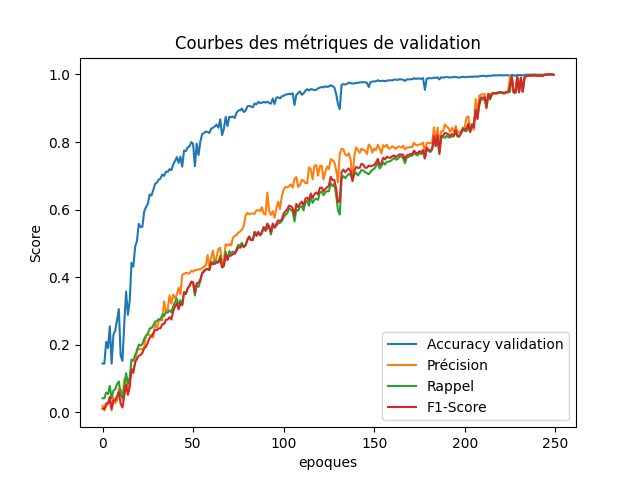
\includegraphics[width=\textwidth]{static/mdl_camembert.png} 
        \caption{Apprentissage (embeddings : Camembert)}
        \label{fig:camenbert}
    \end{minipage}
    \hfill
    \begin{minipage}[b]{0.38\textwidth}
        \centering
        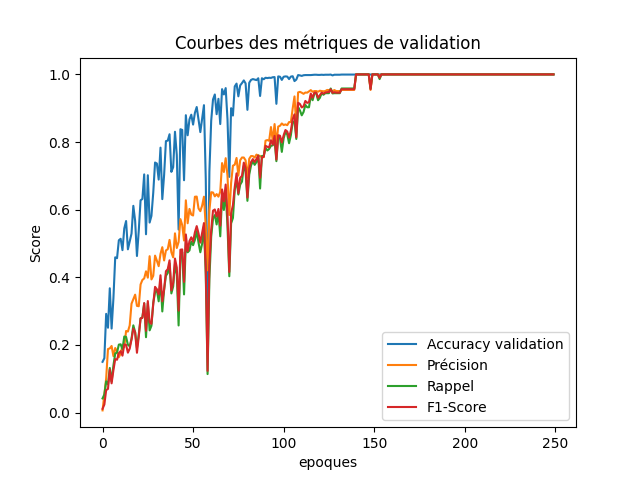
\includegraphics[width=\textwidth]{static/mdl_google_bert.png} 
        \caption{Apprentissage (embeddings : Google Bert)}
        \label{fig:google_bert}
    \end{minipage}
\end{figure}

Nous constatons que la courbe d'évaluation  du mlp sur les embeddings de google bert bien qu'augmentant plus rapidement, est
beaucoup moins régulière que la courbe d'apprentissage du mlp sur les embeddings Camembert. Cela provient probablement du fait 
que le modèle base de Google est un modèle entraîné pour du multi-lingue ce qui n'est pas le cas du modèle Camembert spécifiquement 
entraîné sur des données françaises. C'est différences de performances lors de l'apprentissage suggèrent que le modèle français génère 
des embeddings plus réguliers et traduisant mieux le contexte, que le modèle de google qui lui nécessite un mlp ajusté plus finement afin 
de lisser ces imprécisions sur les embeddings.


\section{K plus proches voisins}

Dans cette partie nous nous penchons sur une approximation de notre modèle précédent, en effet les modèles Bert sont connus 
pour la pertinence des embeddings qu'ils produisent dans un context donné. Comme ces embeddings agglomèrent l'information sur 
le mot et son context il se pourrait qu'ils suffisent à eux seuls à classifier nos mots. Pour cela nous utilisons l'algorithme
des k plus proches voisins qui vise à attribuer la classe majoritaire parmi les voisins du mots que l'on cherche à classifier. Une des premières étapes a été de trouver le nombre 

\subsection{Répartition des données et impact}
\begin{figure}[H]
    \centering
    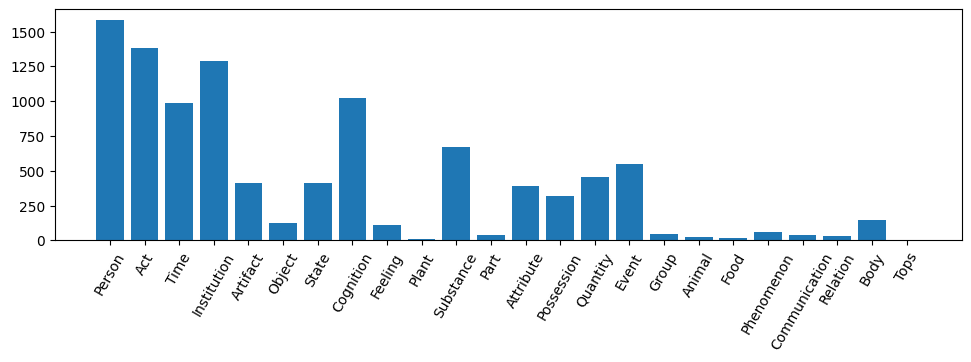
\includegraphics[width=0.8\textwidth]{static/data_rep.png}
\end{figure}

Une analyse de nos données d'entraînement nous donne le graphique ci-dessus, nous avons masqué la classe '*' étant donné que nous
n'évaluons pas les performances sur la prédiction cette classe étant donné qu'elle est grandement majoritaire ( 80\% des exemples d'entraînement) ce qui
fausserait la prédiction. Malgré cela nous constatons tout de même de forte disparités au sein des classes. Nous savons que cela 
influence négativement les performances des différents classifieurs, un dataset plus équilibré serait donc souhaitable si l'on souhaite améliorer
nos performances. 
\begin{figure}[H]
    \centering
    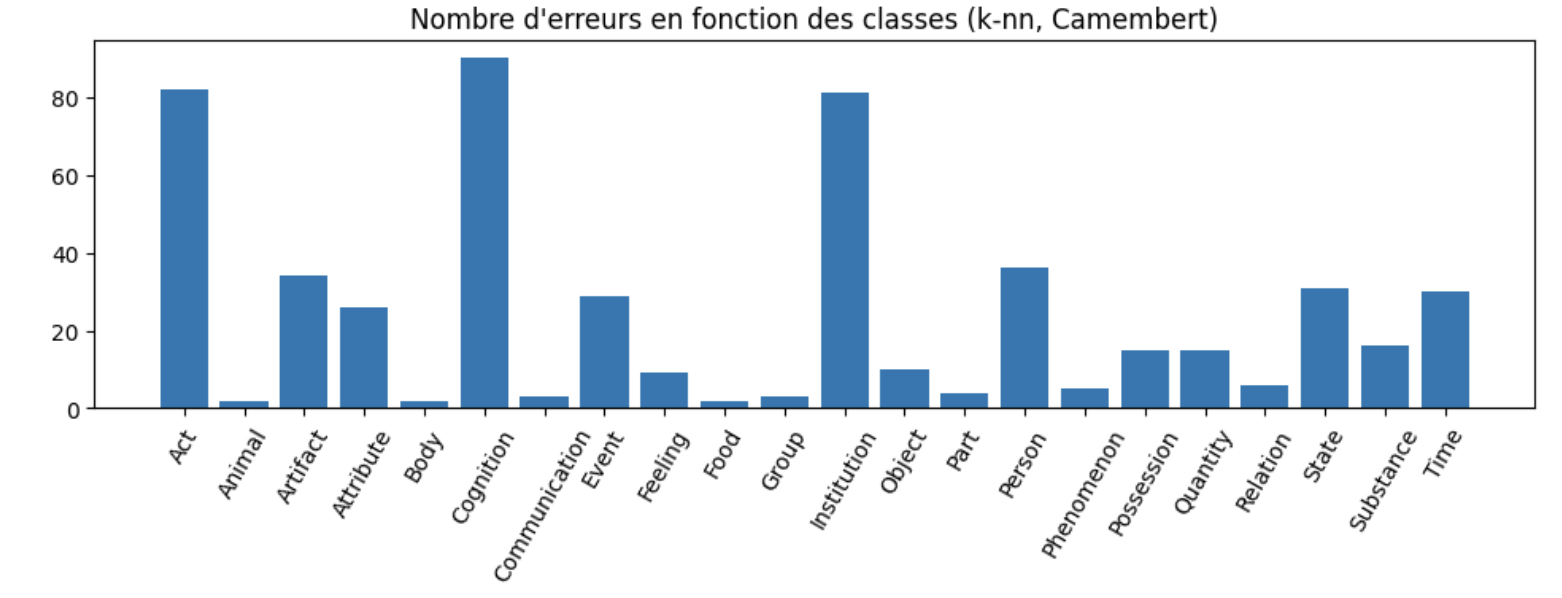
\includegraphics[width=0.8\textwidth]{static/stat_error.png}
\end{figure}

Nous remarquons un avantage sur le k-nn : la répartition des classes ne semble pas avoir un fort impact sur 
les prédictions du modèles contrairement à ce qui est connu pour les réseaux profond (qui commettent beaucoup d'erreurs sur les classes très minoritaires).
\section{Comparaison des performances en fonction de la quantité de données d'apprentissage}


Dans cette partie nous allons nous intéresser à l'influence de la quantité de données lors de l'apprentissage 
de nos modèles sur leurs performances. En effet les tâches de labelisation de données pouvant être complexes et coûteuses
il est intéressant d'étudier la quantité de données nécessaire à un certain type de modèle pour atteindre un certain niveau 
de performances.
\subsection{Comparaison}
Pour cela nous partons toujours du dataset d'entraînement et nous créons des sous échantillons de proportions 
différentes (entre 20\% et 100\% du dataset). Nous réalisons 5 expériences pour chacune de ces proportions et comparons les 
résultats en généralisation. Pour des raisons de temps de calcul, les entraînement seront plafonnés à 20 epochs et non 250 comme 
dans la partie précédente.

\subsubsection{Perceptron Multi Couches}

\begin{figure}[H]
    \centering
    \begin{minipage}[b]{0.45\textwidth}
        \centering
        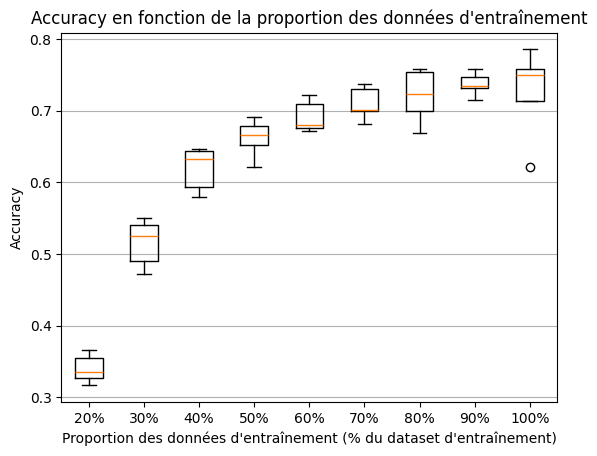
\includegraphics[width=\textwidth]{static/stat_MLP_cam.png} 
        \caption{Apprentissage (embeddings : Camembert)}
        \label{fig:camenbert}
    \end{minipage}
    \hfill
    \begin{minipage}[b]{0.45\textwidth}
        \centering
        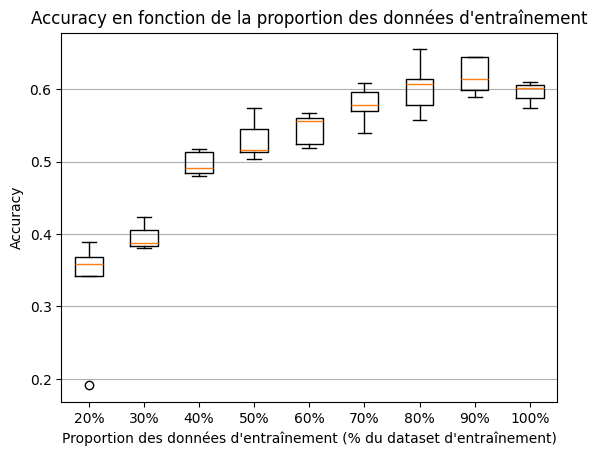
\includegraphics[width=\textwidth]{static/stat_MLP_goo.png} 
        \caption{Apprentissage (embeddings : Google Bert)}
        \label{fig:google_bert}
    \end{minipage}
\end{figure}

La figure ci-dessus représentant les diagrammes en boîtes de nos expériences révèlent quelques points importants. 
Comme nous pouvions nous y attendre la performance augmente avec le nombre de données utilisées lors de l'entraînement,
pour 20\% des données  les résultats oscillent entre 19\% d'accuracy ( pour un outlier) et 40\%. Nous observons une augmentation 
jusqu'à 75\% en moyenne pour un entraînement sur toutes les données disponibles pour les embeddings Camembert et 60\% pour les 
embeddings google. Nous remarquons aussi une courbe moins régulière pour le modèle de google probablement pour les mêmes raisons que 
mentionnées dans la partie 1.1.1.

Comme vu dans les figures 1 et 2, augmenter le nombre de d'itérations lors de l'entraînement augmenterait l'accuracy 
de nos modèles, cependant comme nous n'utilisons que peu de données lors de l'entraînement le risque d'overfitting serait augmenté.
\subsubsection{K plus proches voisins}

A la suite de diverses expériences pour déterminer le $k$ optimal (cf annexes), nous avons observé que prendre en 
compte un nombre élevé de voisins dans la prédiction conduisait à de moins bonnes performances. Dans la suite de cette 
partie nous utiliserons donc k=2. Dans le graph suivant : les échantillons de données sont tirés aléatoirement dans le jeu
de données d'entraînement ce qui induit de légères variations de performances.

\begin{figure}[H]
    \centering
    \begin{minipage}[b]{0.45\textwidth}
        \centering
        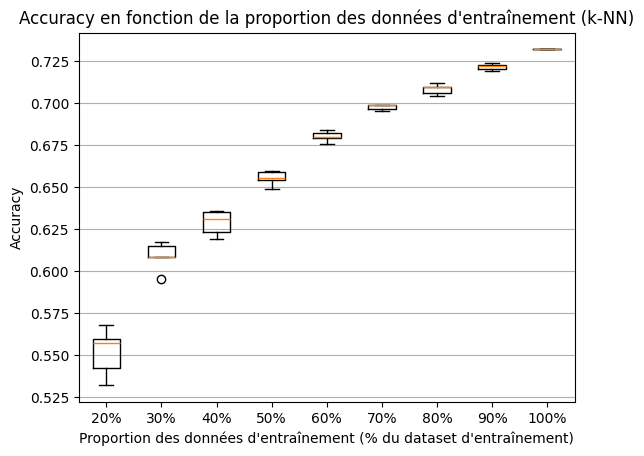
\includegraphics[width=\textwidth]{static/knn_cam_2.png} 
        \caption{Apprentissage (embeddings : Camembert)}
        \label{fig:camenbert}
    \end{minipage}
    \hfill
    \begin{minipage}[b]{0.45\textwidth}
        \centering
        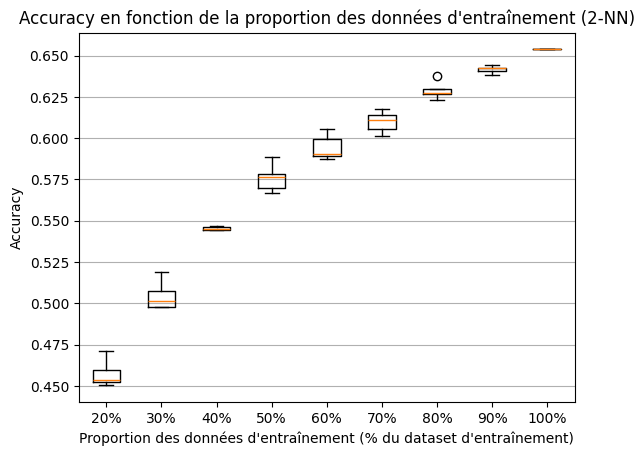
\includegraphics[width=\textwidth]{static/knn_goo_2.png} 
        \caption{Apprentissage (embeddings : Google Bert)}
        \label{fig:google_bert}
    \end{minipage}
\end{figure}

Nous constatons que ce modèle est bien plus performant pour de très faible quantités de données 
d'entraînement, et les performances sur l'ensemble du dataset se rapprochent très fortement de celles 
obtenues avec le perceptron multi-couche (entraîné en 20 epochs). Les résultats montrent aussi que l'apprentissage 
d'un k-nn est plus régulier sur le mlp sur les embeddings générés par google bert.

\section{Conclusion}

Toutes ces expériences mettent divers points intéressant en lumière : 
- le mlp se montre bien plus performant que le k-nn si on l'entraîne avec de bons hyper-paramètres
et que nous avons une quantité de données suffisante et si possible présentant une répartition des classes équilibrée.
- le k-nn obtient de manière acceptable lorsque l'on a très peu de données et semble moins sensible à la répartition des classes
Ainsi nous avons montré que dans la tâche de prédiction de super-senses les deux approches sont possibles et fournissent des résultats aux 
avantages variés. Nous pourrons aussi remarquer que le k-nn à l'avantage d'être un algorithme plus facile à interpréter qu'un mlp néanmoins 
il se montre moins rapide lors de l'inférence lorsque la quantité de vecteurs est importante. 

\renewcommand{\refname}{Bibliographie}
\bibliographystyle{plain}
\bibliography{bibliographie.bib} 

\section{Annexes}

\subsection{K-NN, embeddings Camembert}


\begin{figure}[H]
    \centering
    \begin{subfigure}[t]{0.35\textwidth}
        \centering
        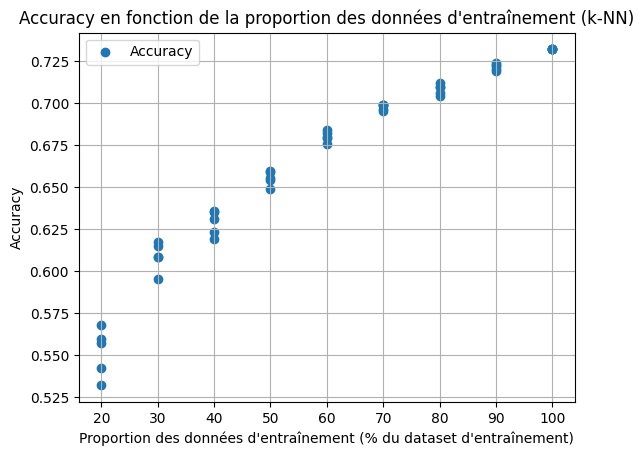
\includegraphics[width=\textwidth]{static/knn_cam_2_raw.png} 
        \caption{Résultat brut k=2}
    \end{subfigure}
    \hfill
    \begin{subfigure}[t]{0.35\textwidth}
        \centering
        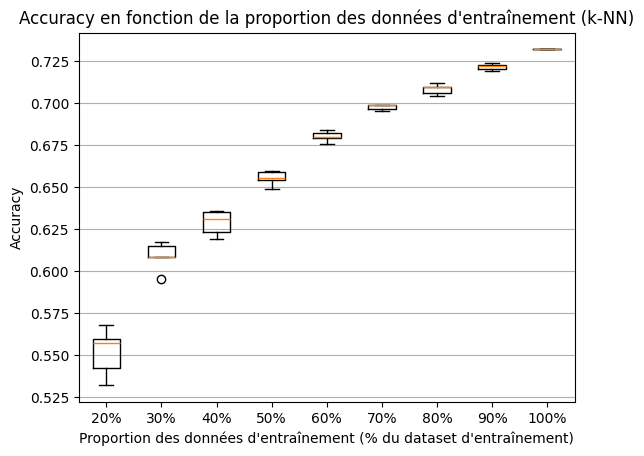
\includegraphics[width=\textwidth]{static/knn_cam_2.png}
        \caption{box plot k=2}
    \end{subfigure}
    \hfill
    \begin{subfigure}[t]{0.35\textwidth}
        \centering
        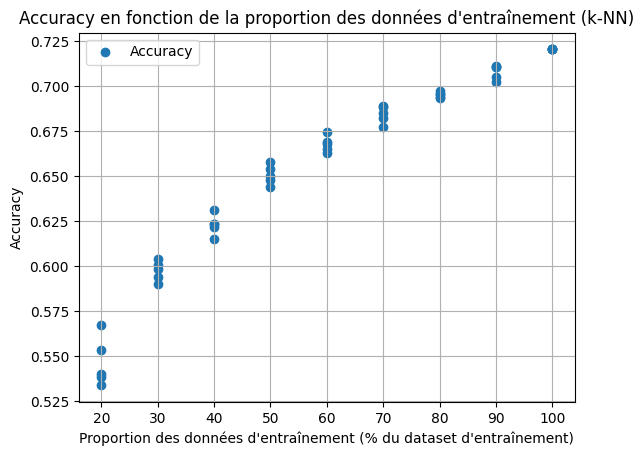
\includegraphics[width=\textwidth]{static/knn_cam_5_raw.png}
        \caption{Résultat brut k=5}
    \end{subfigure}
    \hfill
    \begin{subfigure}[t]{0.35\textwidth}
        \centering
        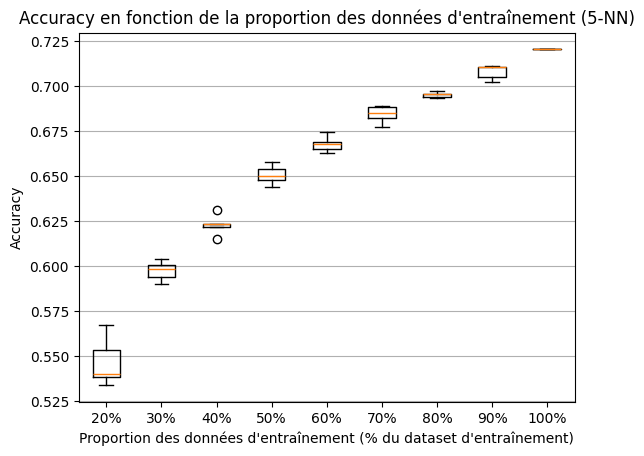
\includegraphics[width=\textwidth]{static/knn_cam_5.png}
        \caption{box plot k=5}
    \end{subfigure}
    \hfill
    \begin{subfigure}[t]{0.35\textwidth}
        \centering
        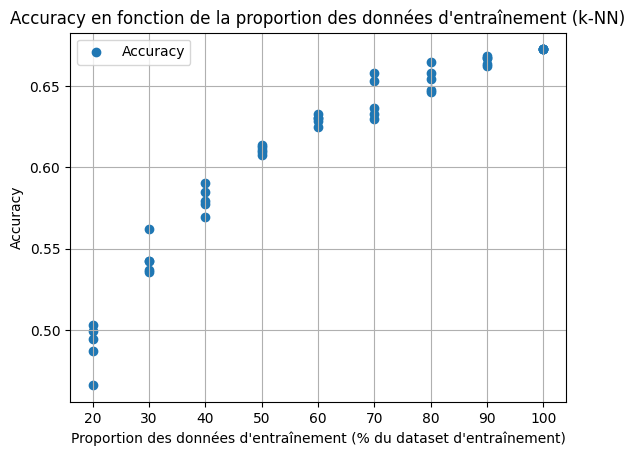
\includegraphics[width=\textwidth]{static/knn_cam_10_raw.png}
        \caption{Résultat brut k=10}
    \end{subfigure}
    \hfill
    \begin{subfigure}[t]{0.35\textwidth}
        \centering
        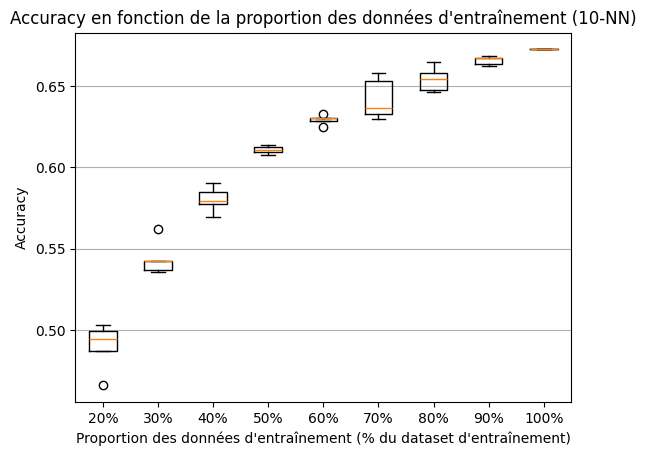
\includegraphics[width=\textwidth]{static/knn_cam_10.png}
        \caption{box plot k=10}
    \end{subfigure}
    \hfill
    \begin{subfigure}[t]{0.35\textwidth}
        \centering
        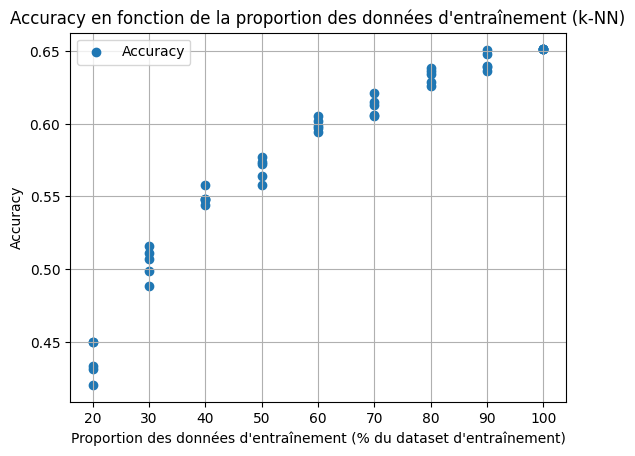
\includegraphics[width=\textwidth]{static/knn_cam_15_raw.png}
        \caption{Résultat brut k=15}
    \end{subfigure}
    \hfill
    \begin{subfigure}[t]{0.35\textwidth}
        \centering
        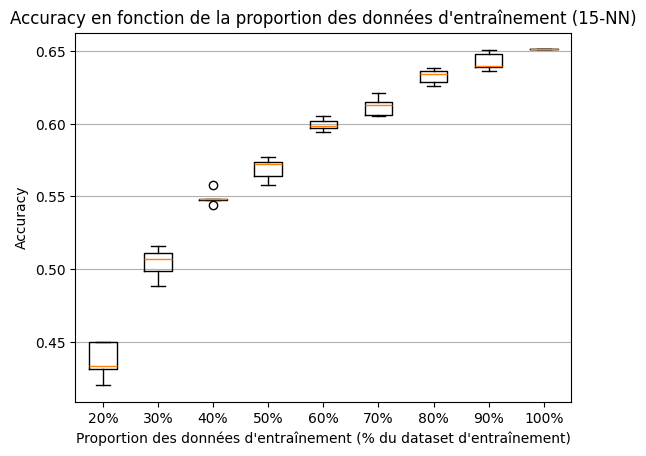
\includegraphics[width=\textwidth]{static/knn_cam_15.png}
        \caption{box plot k=15}
    \end{subfigure}

    \caption{Expériences pour déterminer le nombre de voisins à utiliser}
\end{figure}



\subsection{K-NN, embeddings Google Bert}
\begin{figure}[H]
    \centering
    \begin{subfigure}[t]{0.35\textwidth}
        \centering
        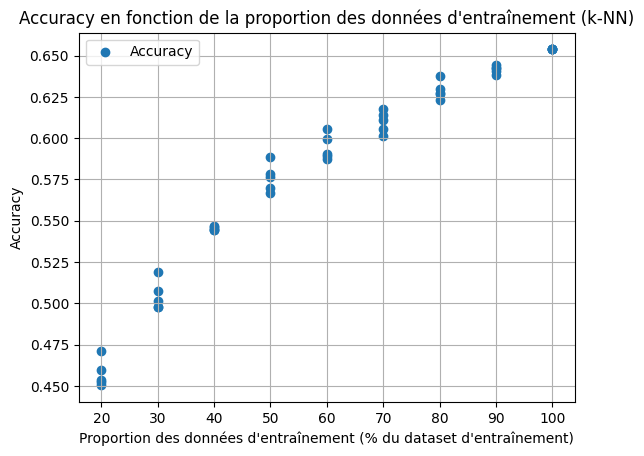
\includegraphics[width=\textwidth]{static/knn_goo_2_raw.png} 
        \caption{Résultat brut k=2}
    \end{subfigure}
    \hfill
    \begin{subfigure}[t]{0.35\textwidth}
        \centering
        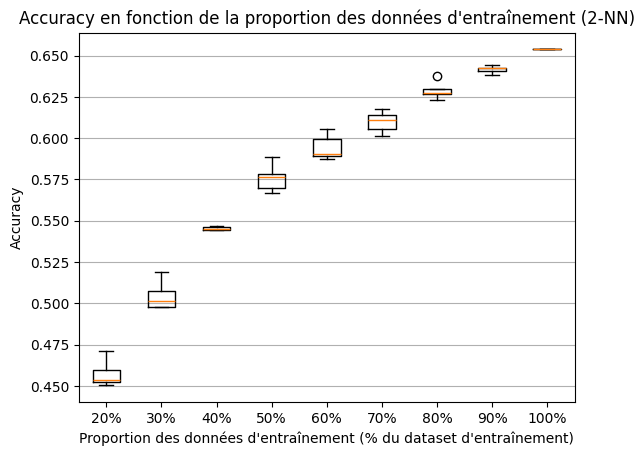
\includegraphics[width=\textwidth]{static/knn_goo_2.png}
        \caption{box plot k=2}
    \end{subfigure}
    \hfill
    \begin{subfigure}[t]{0.35\textwidth}
        \centering
        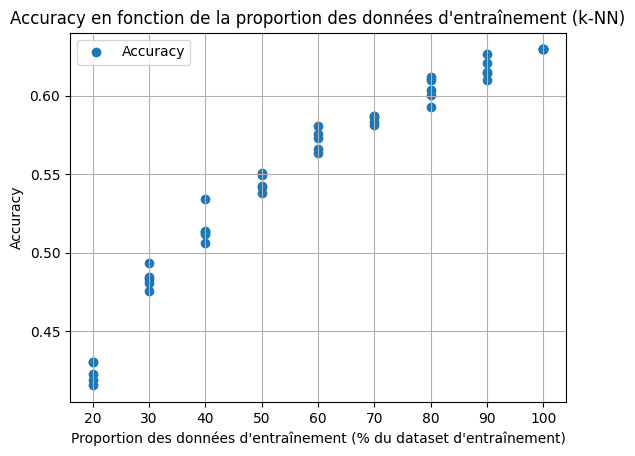
\includegraphics[width=\textwidth]{static/knn_goo_5_raw.png}
        \caption{Résultat brut k=5}
    \end{subfigure}
    \hfill
    \begin{subfigure}[t]{0.35\textwidth}
        \centering
        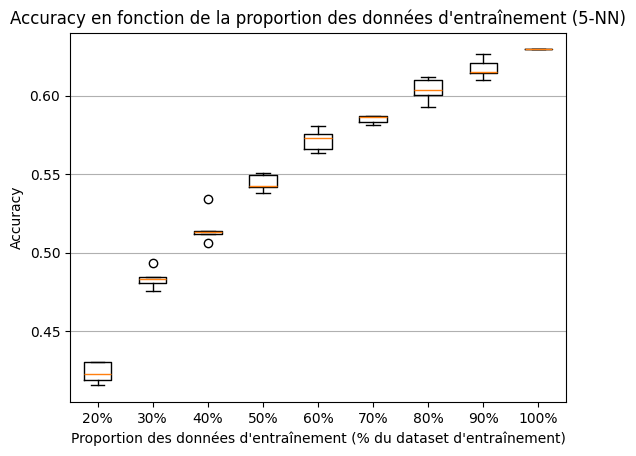
\includegraphics[width=\textwidth]{static/knn_goo_5.png}
        \caption{box plot k=5}
    \end{subfigure}
    \hfill
    \begin{subfigure}[t]{0.35\textwidth}
        \centering
        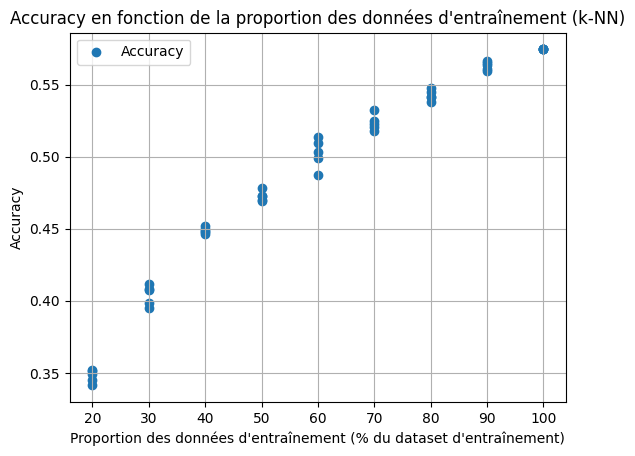
\includegraphics[width=\textwidth]{static/knn_goo_10_raw.png}
        \caption{Résultat brut k=10}
    \end{subfigure}
    \hfill
    \begin{subfigure}[t]{0.35\textwidth}
        \centering
        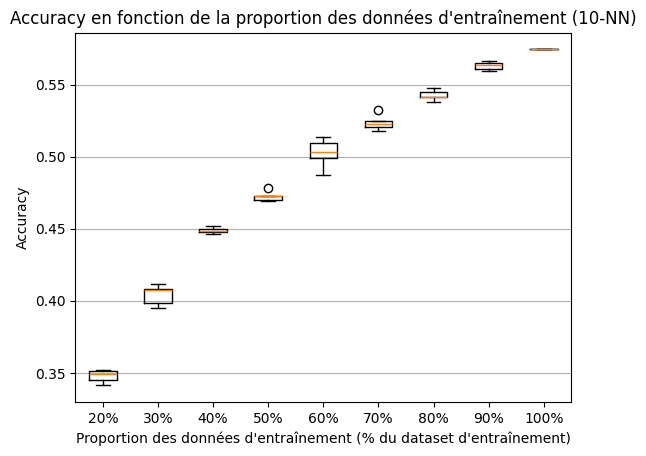
\includegraphics[width=\textwidth]{static/knn_goo_10.png}
        \caption{box plot k=10}
    \end{subfigure}

    \caption{Expériences pour déterminer le nombre de voisins à utiliser}
\end{figure}



\end{document}
